\subsection{Evaluation: ANN vs. linear regression models}
\label{sec:linreg_evaluation}
In this section, we statistically evaluate if there is a significant performance difference between the linear regression models and the ANN. The evaluation will be based on a t-test analysis and analyzing the credibility interval for the different models.

For the t-test, we test the hypothesis of the difference in prediction error could happen by coincidence, with the threshold $\alpha = 0.05$. The procedure follows the method for the general solution for model evaluation as seen in section 9.3.1 in the course notes \cite{coursenotes}.

For the ANN and linear regression model, we get a p-value for the t-test to be 0.824. This is larger than $\alpha$, and therefore we cannot reject the hypothesis. Calculating the credibility interval for the difference of the prediction errors of the two models, we get the interval $[-4.59\cdot10^{-6}, 7.80\cdot10^{-6}]$ meaning the difference of error is of 95\% of probability within this interval. Since 0 is within the interval, the two models cannot be declared significantly different, thus confirming the result from the t-test.


%(i.e., considering the credibility interval equivalent to the use of a paired t-test as described in lecture 6 and last exercise week 6). Compare in addition if the performance of your models are better than simply predicting the output to be the average of the training data output.

%Are the models better than predicting the output as the average of the training data output?

Comparing the two models with a model which always predicts the average training value of the refractive index we get p-values with order of magnitude around $10^{-4}$, showing that both models are significantly different from predicting the output as the mean value. Like before, we can check the credibility intervals between the ANN, linear regression and the model always predicting the mean value. The intervals are: $[-1.84\cdot10^{-4}, -1.34\cdot10^{-4}]$ and $[-1.83\cdot10^{-4}, -1.38\cdot10^{-4}]$ respectively. Both intervals completely span negative values, which tells us, that the two models are significantly different from the mean predicting model as 0 is not in the intervals. Also we see that the mean predicting model's errors are more severe since the intervals are negative. This result was expected from the previous sections when analyzing the regression models. 


\begin{figure}[H]
    \centering
    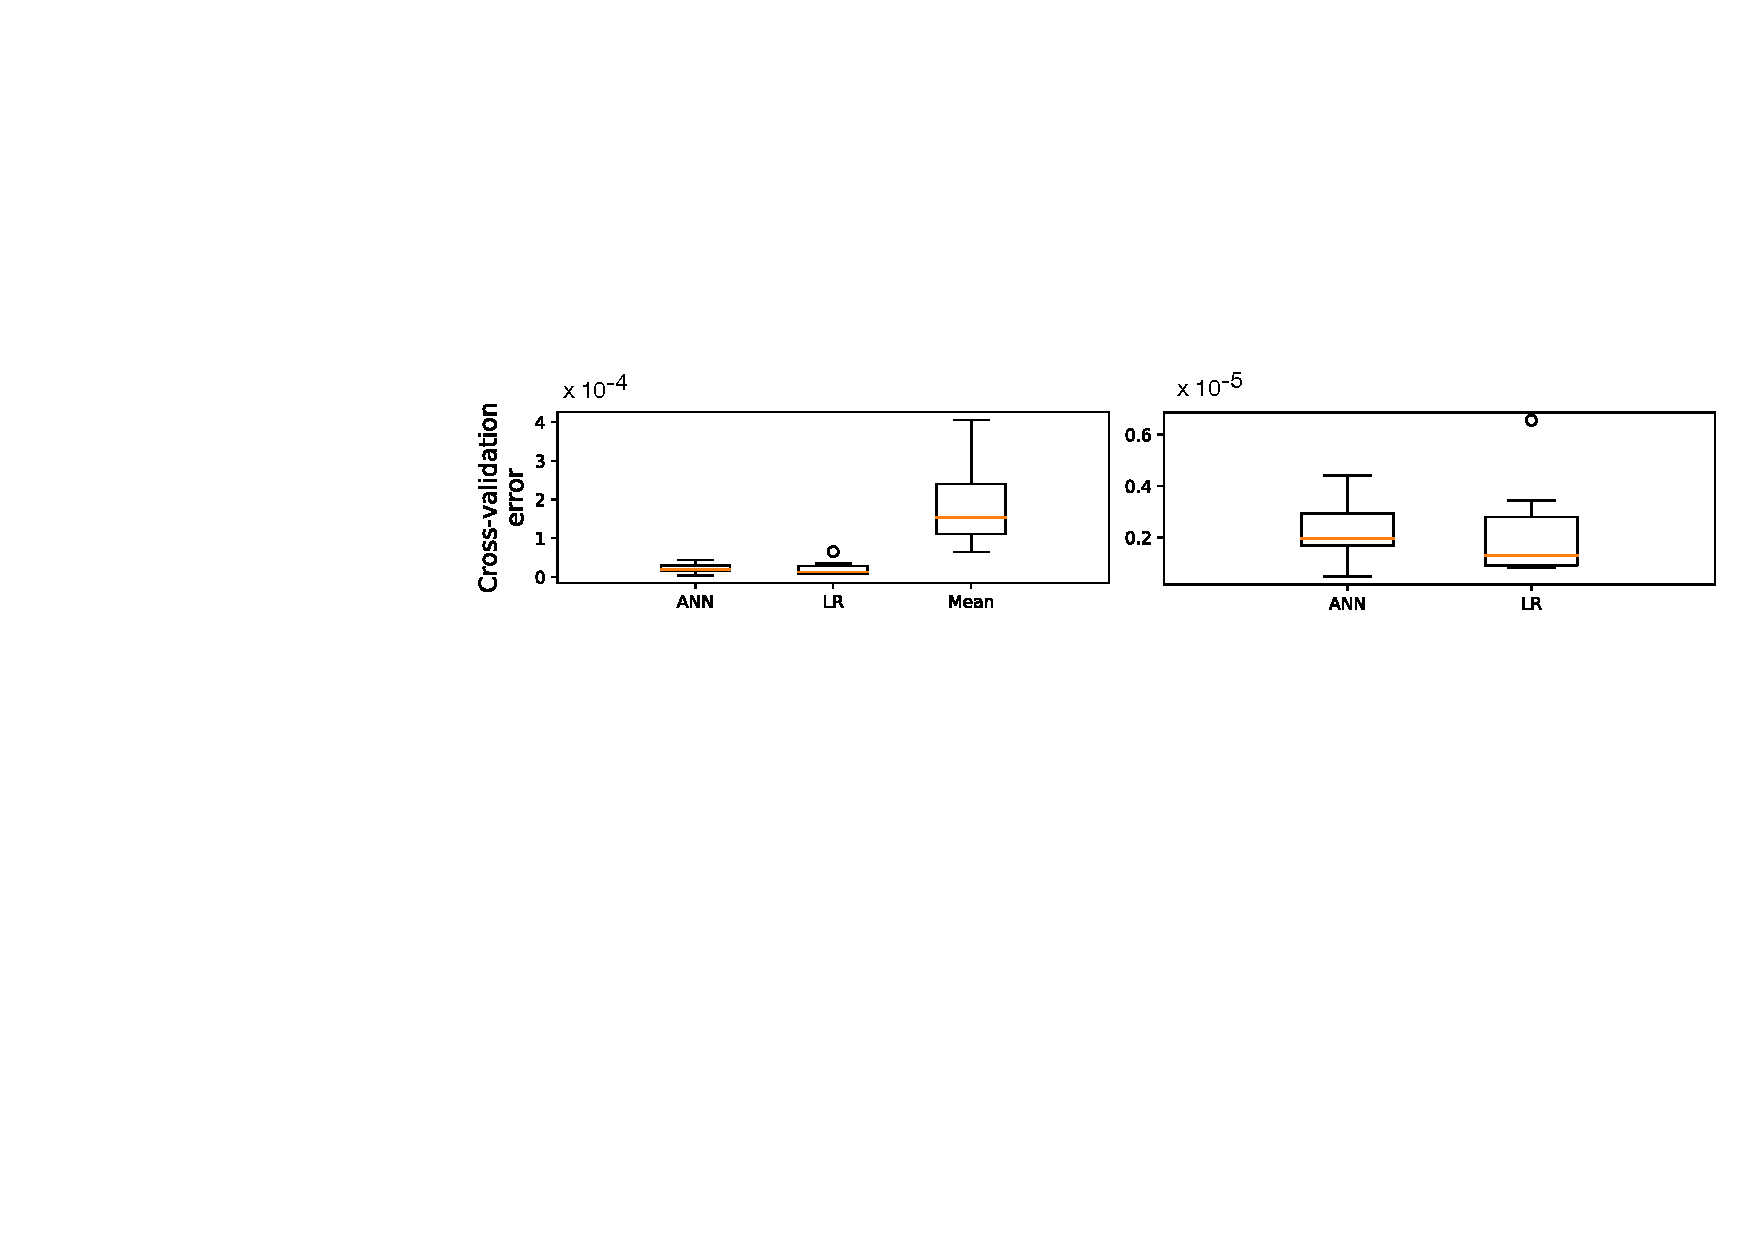
\includegraphics[width=\textwidth]{fig/RegressionEvaluationBoth.pdf}
    \caption{Comparisons of the prediction errors obtained by cross validation between the three models: Linear regression, Artificial neural network and a model which always predicts the mean value. The right plot neglects the mean predicting model.}
    \label{fig:cv_reg}
\end{figure}


Comparisons of the cross-validation errors between the two regression models and the mean predicting model are seen in figure \ref{fig:cv_reg}. It is safe to say that the two regression models perform better the mean predicting model. But as the tests showed, we cannot say which of the two regression models have the best performance.
